\documentclass[11pt]{beamer}
\usetheme{Antibes}
\usepackage[utf8]{inputenc}
\usepackage[german]{babel}
\usepackage[T1]{fontenc}
\usepackage{amsmath}
\usepackage{amsfonts}
\usepackage{amssymb}
\usepackage{graphicx}
%\author{}
%\title{}
%\setbeamercovered{transparent} 
%\setbeamertemplate{navigation symbols}{} 
%\logo{} 
%\institute{} 
%\date{} 
%\subject{} 
\begin{document}
\section{Messung der Verdampfungsenthalpie}
\begin{frame}{Messung der Verdampfungsenthalpie}
\begin{equation*}
\frac{dp}{dT}=\frac{\nu \Lambda}{T(V_1-V_2)}
\end{equation*}
\begin{equation*}
\ln(p)=-\frac{\Lambda}{R}\cdot \frac{1}{T}+c \text{ mit } c=const
\end{equation*}
\end{frame}

\begin{frame}
\begin{figure}[H]
\centering
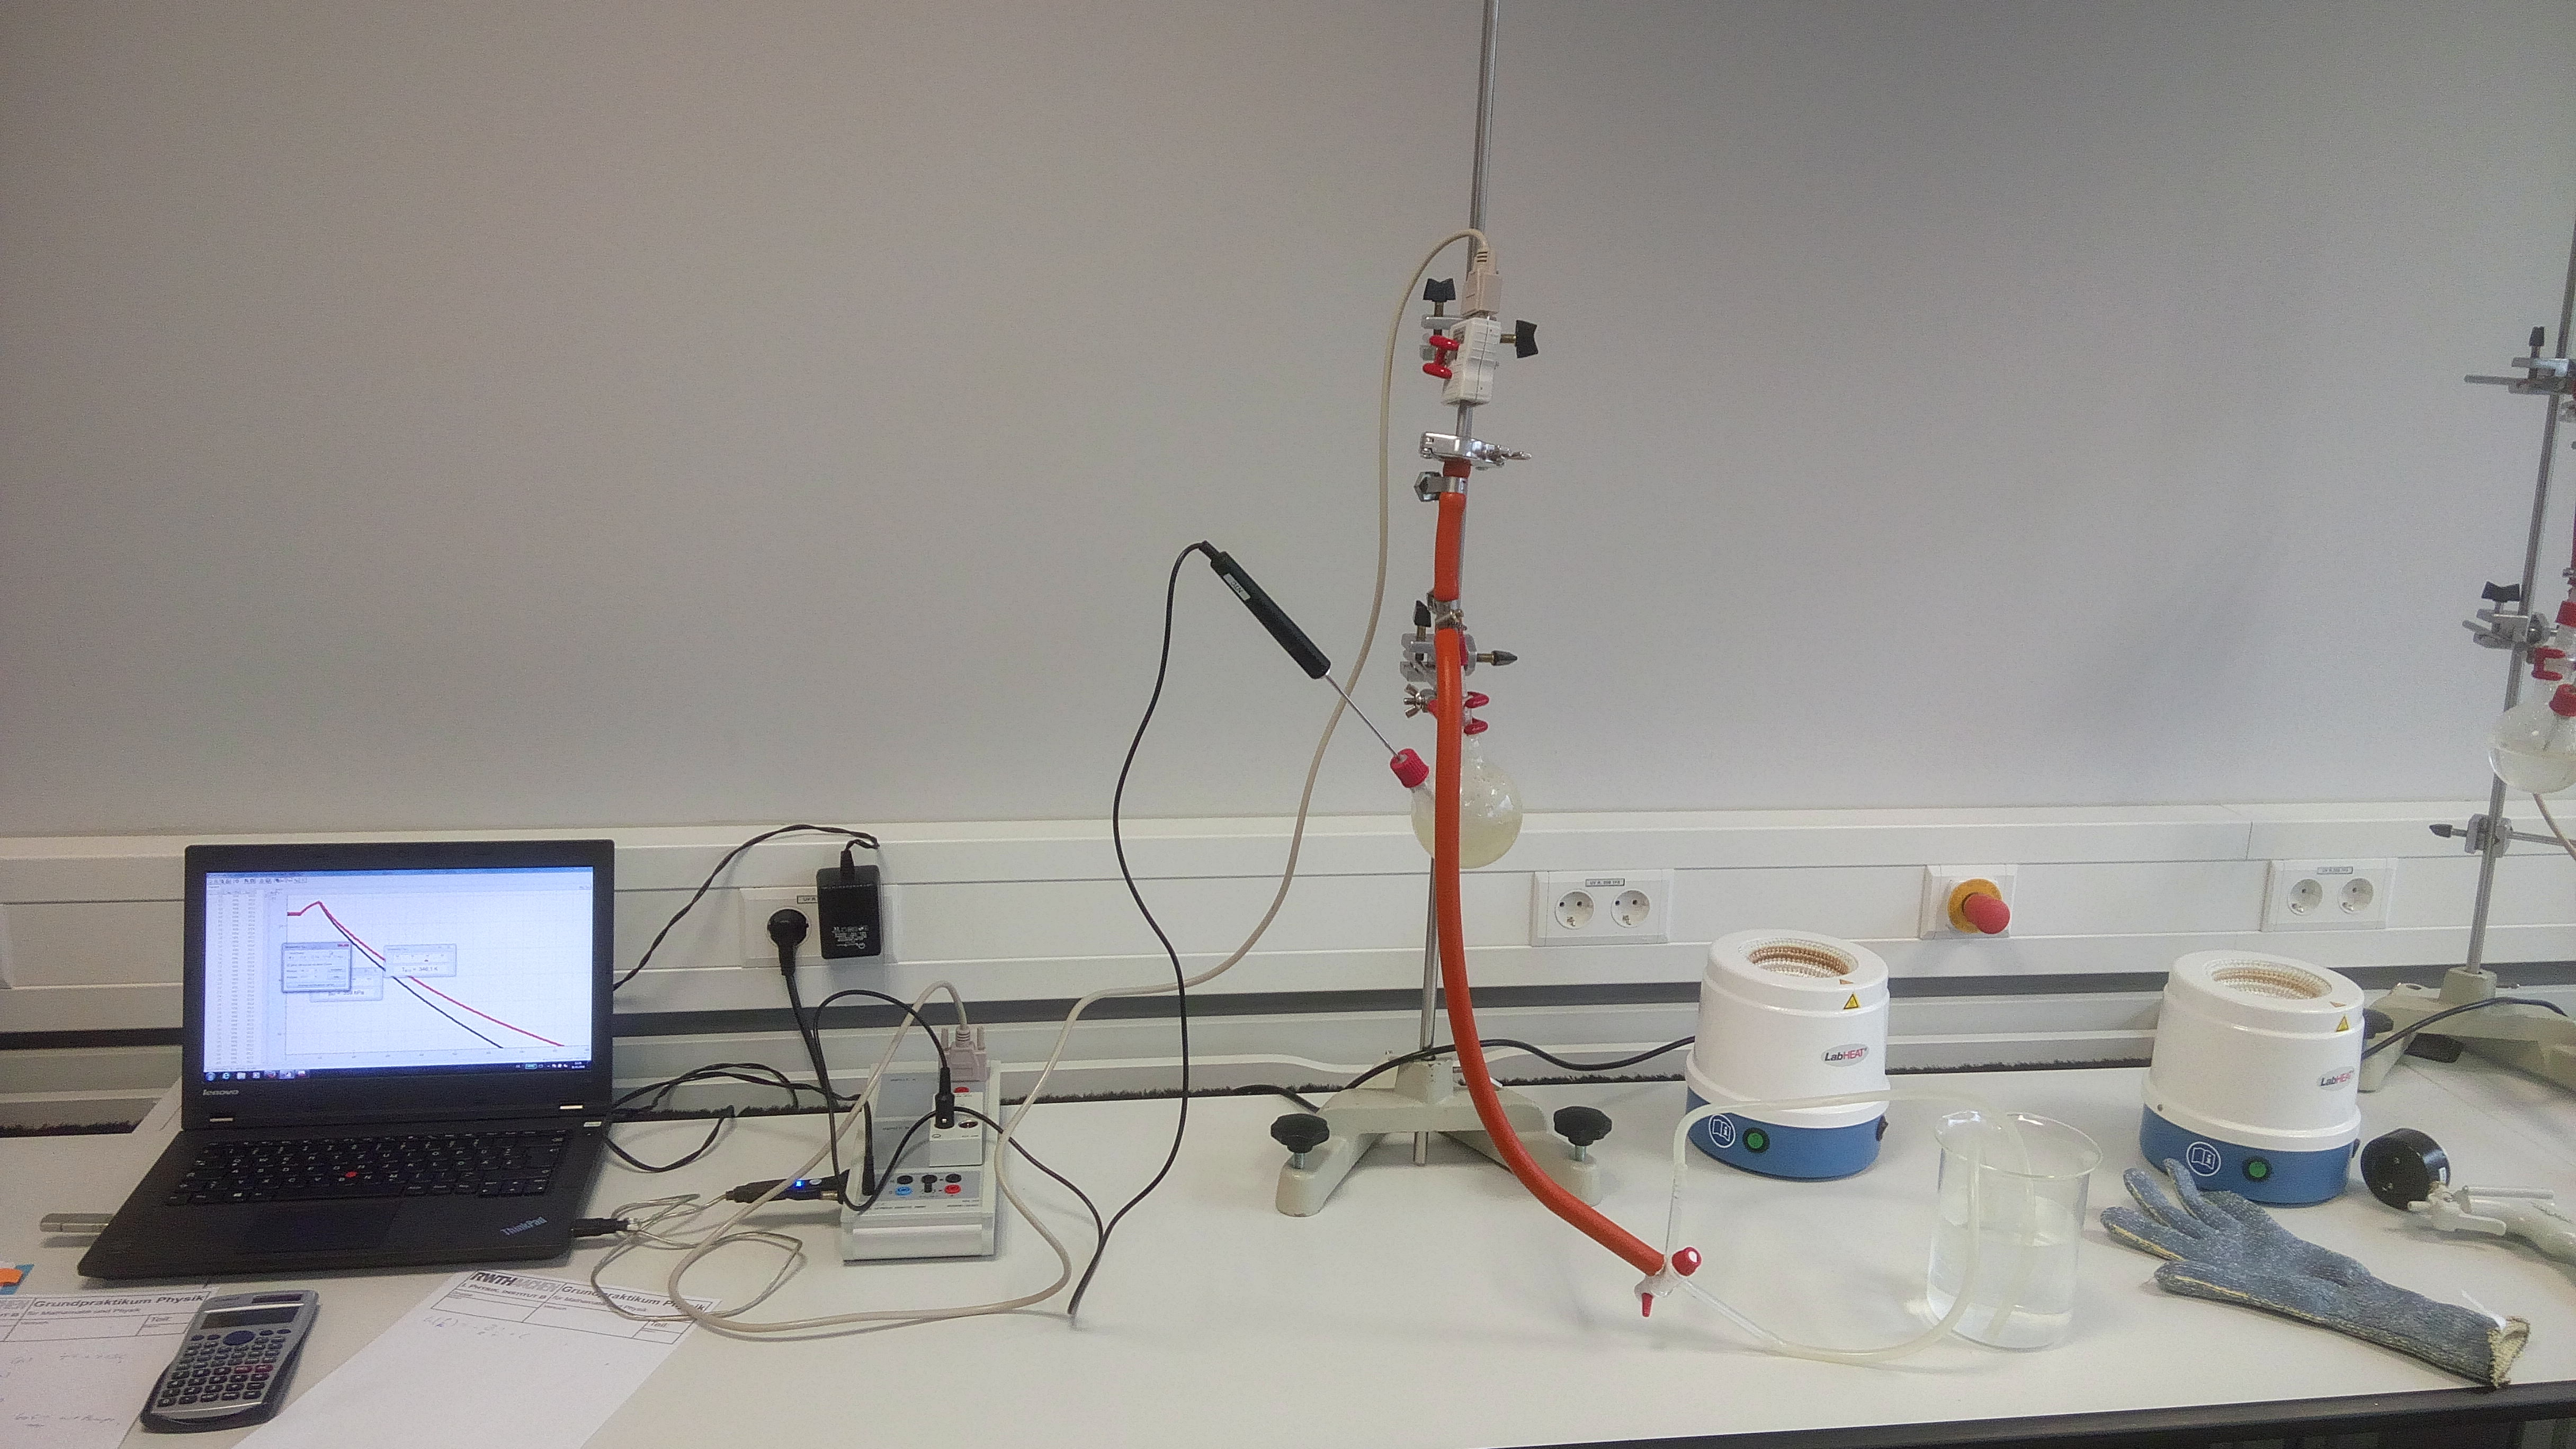
\includegraphics[scale=0.065]{Bilder/IMG_20160331_121650.jpg}
\end{figure}
\end{frame}

\subsection{Rohdaten}
\begin{frame}
\begin{figure}[H]
\centering
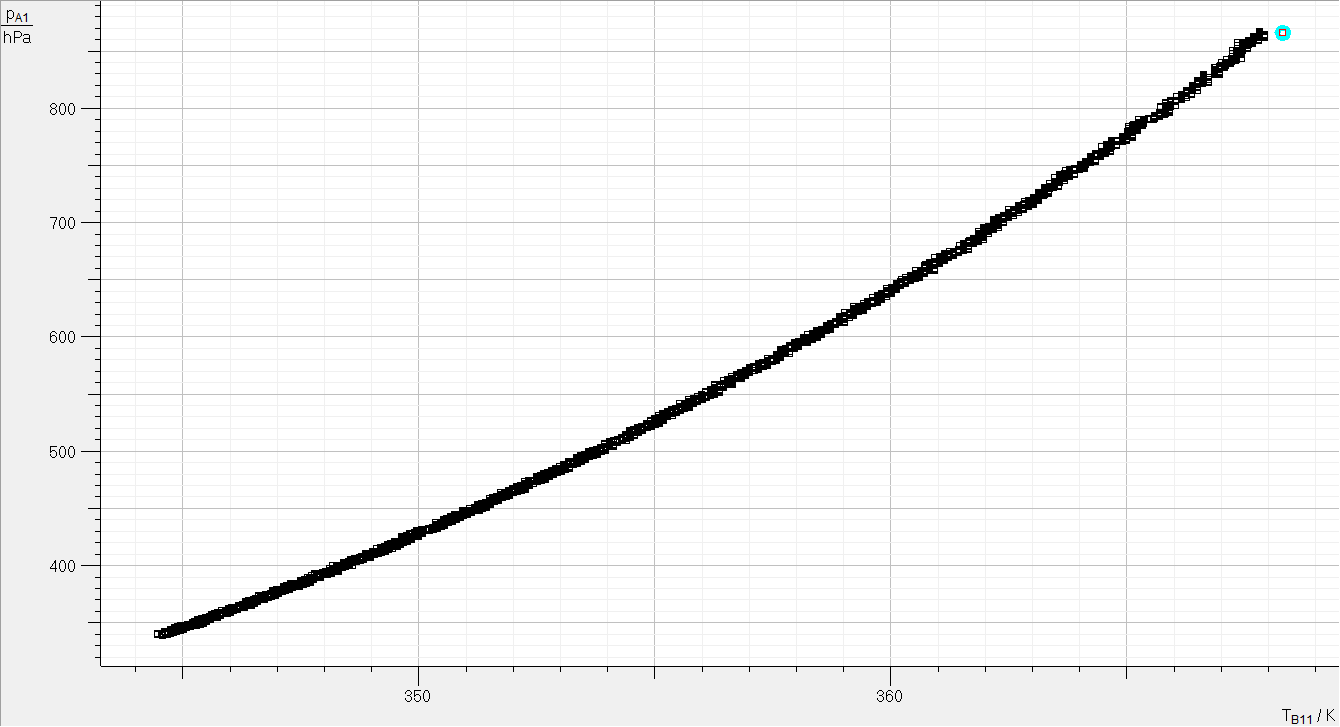
\includegraphics[scale=0.4]{Bilder/RohdatenHaupmessungGrp11.png}
\end{figure}
\end{frame}

\begin{frame}
\begin{figure}[H]
\centering
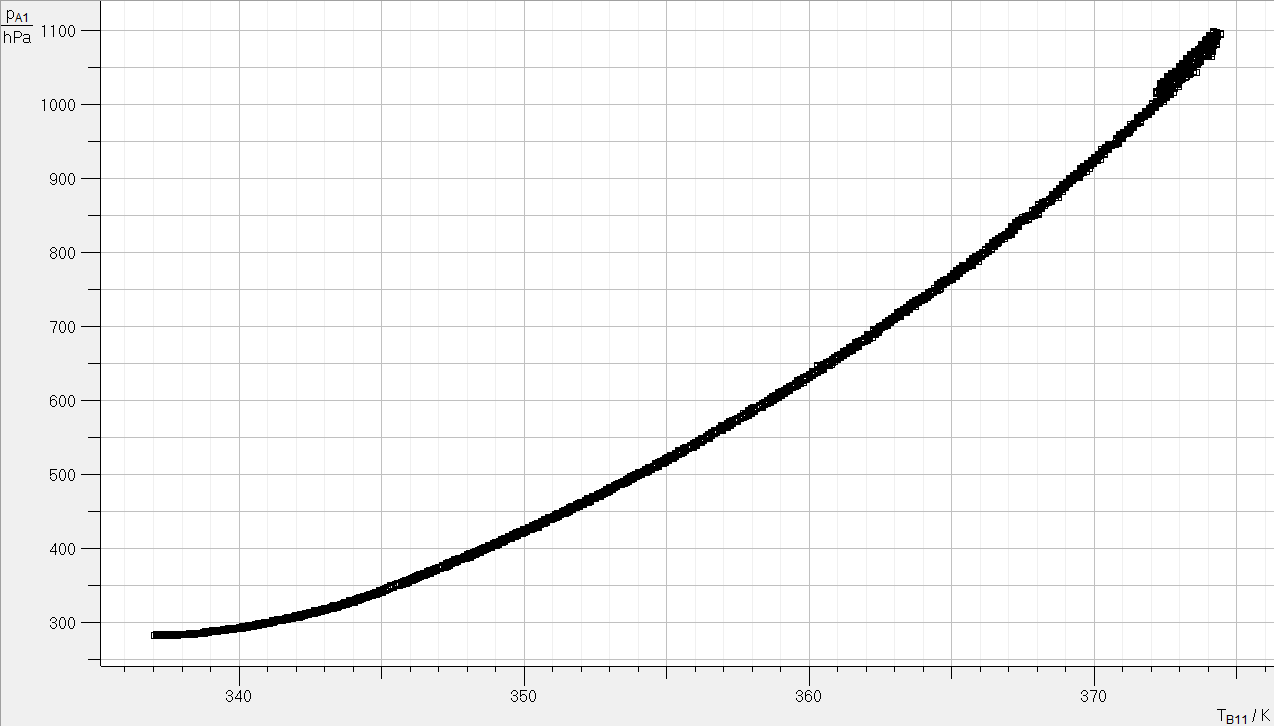
\includegraphics[scale=0.4]{Bilder/RohdatenHaupmessungGrp2.png}
\end{figure}
\end{frame}

\subsection{Transformation der Rohdaten}
\begin{frame}
\begin{figure}[H]
\centering
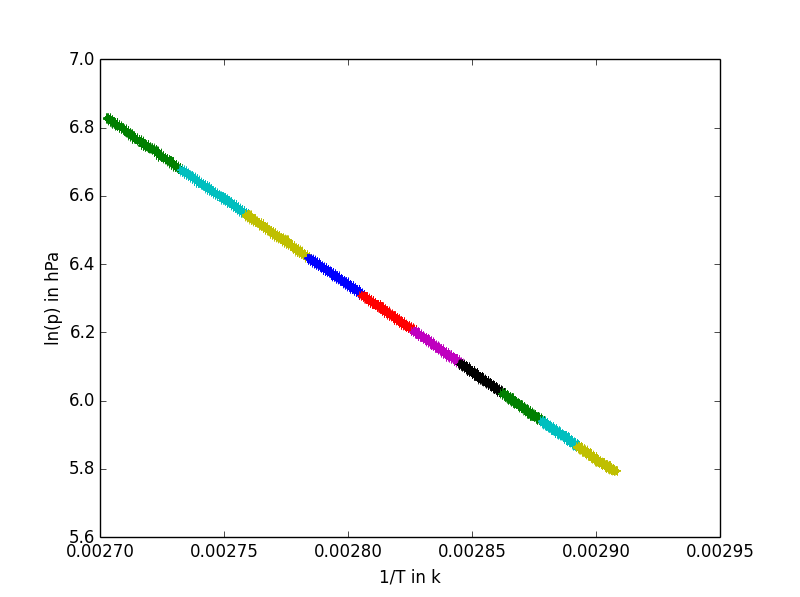
\includegraphics[scale=0.5]{Bilder/linreg_EL_neuerFehler.png}
\end{figure}
\end{frame}

\begin{frame}
\begin{figure}[H]
\centering
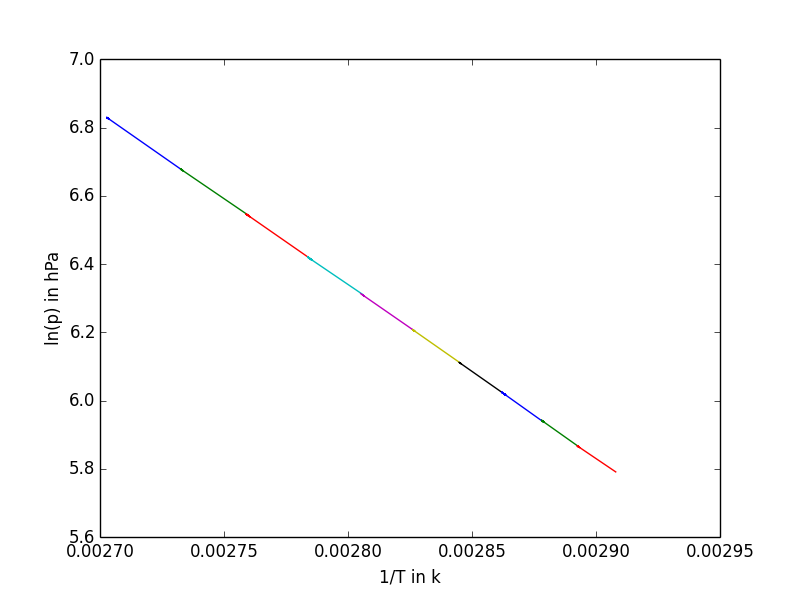
\includegraphics[scale=0.5]{Bilder/linreg_nurlinreg_EL.png}
\end{figure}
\begin{itemize}
\item $\frac{\chi^2}{f} \Rightarrow 1.27 | 0.96 | 1.12 | 0.86 | 0.89 | 0.77 | 0.79 | 0.78 | 0.71 | 0.74$
\end{itemize}
\end{frame}

\subsection{Ergebnisse}
\begin{frame}
\begin{equation*}
\ln(p)=-\frac{\Lambda}{R}\cdot \frac{1}{T}+c \text{ mit } c=const
\end{equation*}
\begin{table}[H]\centering
\begin{tabular}{c|c|c|c|c}
Abschnitt&T in K&$\Lambda$ in $\frac{kJ}{mol}$&$\sigma_{\Lambda_{stat}}$in $\frac{kJ}{mol}$&$\sigma_{\Lambda_{sys}}$in $\frac{kJ}{mol}$\\
\hline
1&367.93&42.18&0.273&0.518\\
2&364.13&41.17&0.156&0.508\\
3&360.76&41.96&0.102&0.518\\
4&357.71&40.97&0.1&0.508\\
5&355.03&41.8&0.12&0.519\\
6&352.6&42.24&0.117&0.525\\
7&350.38&42.31&0.136&0.527\\
8&348.4&43.03&0.141&0.537\\
9&346.54&42.79&0.162&0.535\\
10&344.83&40.84&0.175&0.512\\
\end{tabular}
\end{table}
zum Vergleich - $\Lambda_{Lit}=40.6\,\frac{kJ}{mol}$
\end{frame}

\subsection{Verdampfungswärme gg Temperatur}
\begin{frame}
\begin{figure}[H]
\centering
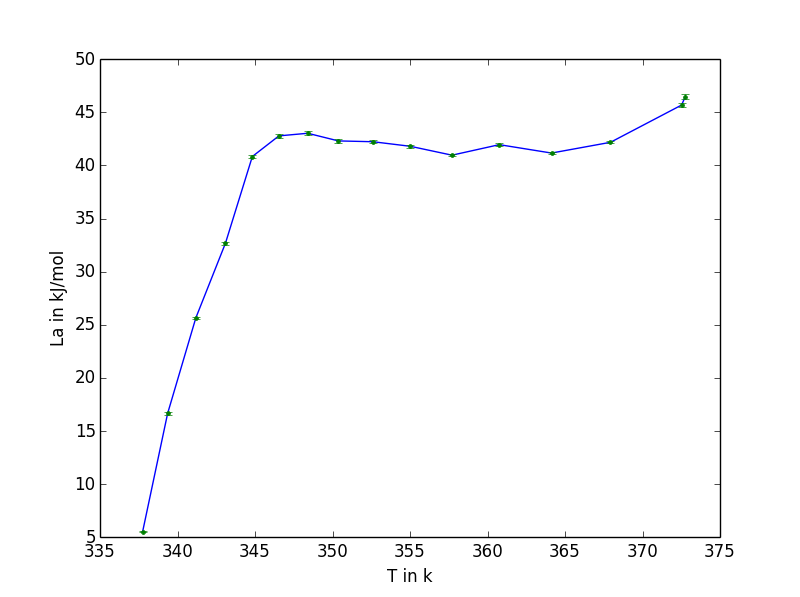
\includegraphics[scale=0.5]{Bilder/lamda_EL_neuerFehler.png}
\end{figure}
\end{frame}

\subsection{Fazit}
\begin{frame}
\begin{itemize}
\item Werte für $\Lambda$ zwischen 1 und 10 $\sigma$ um Literaturwert $40.6 \frac{kJ}{mol}$
\item fallende Verdampfungsenthalpie bei steigender Temperatur konnte verifiziert werden
\end{itemize}
\end{frame}

\end{document}